\documentclass{beamer}
\usepackage{listings}
\usepackage{soul}
\usepackage{color}
\usepackage{enumitem}
\usepackage{amsfonts}
\usepackage[binary-units=true, per-mode=symbol-or-fraction]{siunitx}
\usepackage[loop=true]{animate}
\usepackage{tikz}
\usepackage[ruled,vlined]{algorithm2e}
\usepackage{caption}
\usetikzlibrary{positioning}
\usepackage{booktabs,multirow,tabularx,multicol}
\usepackage{empheq}
\usepackage[many]{tcolorbox}

\renewcommand{\thealgocf}{}

% Bibliography
\usepackage[
  backend=biber,   % use modern biber backend
  firstinits=true,
  date=iso8601,
]{biblatex}
\addbibresource{references.bib}  % die Bibliographie einbinden
% \DefineBibliographyStrings{english}{andothers = {{et\,al\adddot}}}

\setlist[itemize,1]{label=\scriptsize$\blacksquare$}
\setlist[itemize,2]{label= $\diamond$}
\definecolor{mygray}{rgb}{0.8,0.8,0.8}
\definecolor{comments}{RGB}{112,168,193}
\definecolor{stringcolor}{RGB}{43,114,144}
\definecolor{keywords}{RGB}{9, 72, 99}
\definecolor{seedclr}{rgb}{0.76, 0.23, 0.13}
\definecolor{txtclr}{rgb}{0.9, 0.9, 0.9}
\definecolor{arrowclr}{rgb}{0.9, 0.9, 0.9}
\definecolor{emphbg}{rgb}{0.98, 0.81, 0.69}
\definecolor{refclr}{rgb}{0.13, 0.55, 0.13}
\newcolumntype{C}{>{\centering\arraybackslash}X}
\newcolumntype{K}[1]{>{\centering\arraybackslash}p{#1}}
\newcommand{\kn}{$k$}


\lstset{ %
  basicstyle=\fontsize{7pt}{7.4pt}\lstfont,        % the size of the fonts that are used for the code
  breakatwhitespace=true,          % sets if automatic breaks should only happen at whitespace
  breaklines=false,                % sets automatic line
  otherkeywords={repeated},        % if you want to add more keywords to the set
  commentstyle=\color{comments},   % comment style
  keepspaces=true,                 % keeps spaces in text, useful for keeping indentation of code (possibly needs columns=flexible)
  keywordstyle=\color{keywords},   % keyword style
  showspaces=false,                % show spaces everywhere adding particular underscores; it overrides 'showstringspaces'
  showstringspaces=false,          % underline spaces within strings only
  showtabs=false,                  % show tabs within strings adding particular underscores
  stepnumber=4,                    % the step between two line-numbers. If it's 1, each line will be numbered
  stringstyle=\color{stringcolor}, % string literal style
  tabsize=2,                       % sets default tabsize to 2 spaces
}

\tikzset{ %
  ,>=latex
  ,every node/.style={font=\bf}
  ,seed/.style={draw, circle, inner sep=0, minimum size=14pt, node distance=27pt, fill=seedclr, text=txtclr}
  ,ref/.style={draw, circle, inner sep=0, minimum size=14pt, node distance=27pt, fill=refclr, text=txtclr}
  ,vertex/.style={draw, circle, inner sep=0, minimum size=14pt, node distance=27pt}
  ,prob/.style={inner sep=0}
}

\DeclareMathOperator*{\argmax}{arg\,max}
\DeclareMathOperator*{\argmin}{arg\,min}
\DeclareMathOperator*{\avg}{avg\,}

\usetheme{metropolis} % Use metropolis theme

\title{A Referral-reward embedded, bi-phase information diffusion technique}
\date{January 30, 2017}
\author{
\large{Sneha Mondal} \\ \\
M.Sc. (Engg.) Colloquium \\
Faculty Advisor : Prof. Y. Narahari\\
}
\institute{
Department of Computer Science and Automation\\
Indian Institute of Science, Bangalore}

\begin{document}
\maketitle

\begin{frame}{Outline}
\tableofcontents
\end{frame}

\section{Introduction}

% \begin{frame}{Marketing Campaigns on Social Media}
%   %Companies use existing social-network services and other technologies to increase brand awareness, launch advertising campaigns and increase revenue.
%   \begin{itemize}
%     \item Increasingly popular - Ads on YouTube, Facebook, Google
%     \item Effectively exploits homophily and social influence
%     \item Relies on underlying network structure
%   \end{itemize}
%   \begin{columns}
%     \column{0.7\textwidth}
%     \center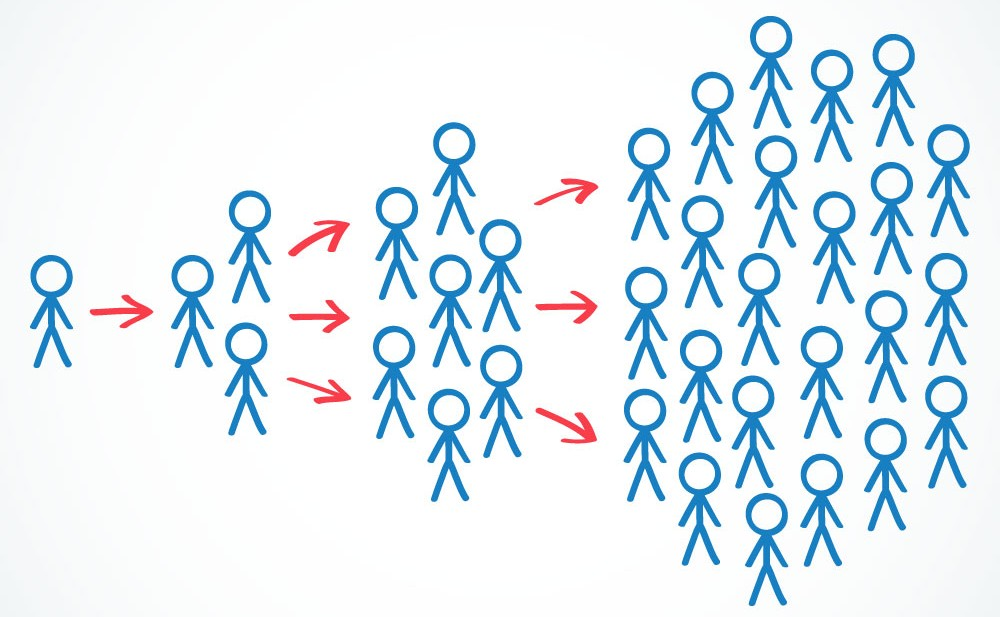
\includegraphics[height=2cm,width=4cm]{IntroPic_1.jpg}
%     \column{0.7\textwidth}
%     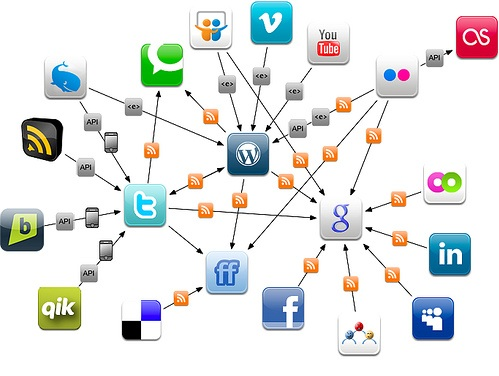
\includegraphics[height=2.5cm,width=4cm]{IntroPic_2.jpg}
%   \end{columns}
% \end{frame}

\begin{frame}{Advertising Campaigns on Social Media}
  \begin{columns}
    \column{0.5\textwidth}
    \begin{itemize}
      \item<1-> {\color{orange}{\textbf{Diffusion via word-of-mouth}}}
      \only<1>{\\Identify initial adopters. Word-of-mouth influence propagation}
      \item<2-> {\color{orange}{\textbf{Referral Rewards}}}
      \only<2>{\\Refer product to friends and acquaintances. Get incentives for successful referral}
    \end{itemize}
    \column{0.6\textwidth}
    \only<1>{\center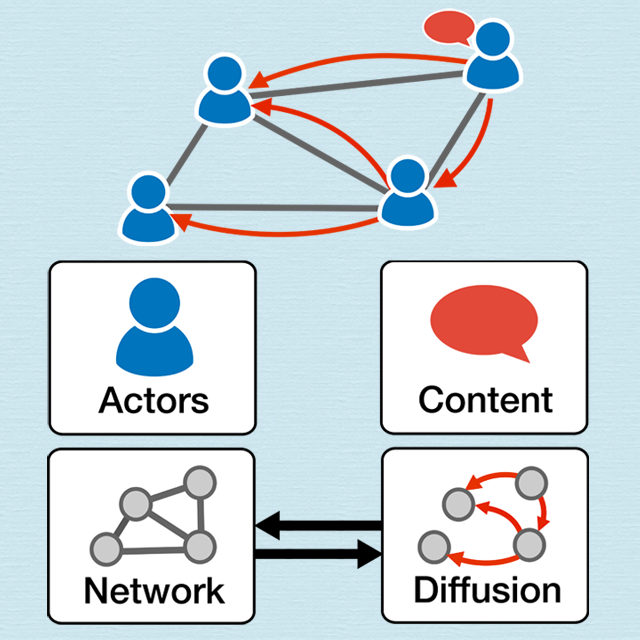
\includegraphics[height=5cm]{informationdiff.png}}
    \only<2>{\center
\includegraphics[height=5cm]{referral.png}}
  \end{columns}
\end{frame}

\begin{frame}{Problem Setting}
  \begin{itemize}
    \item {\color{orange}{Given}}
    \begin{itemize}
      \item Target consumer base
      \item Estimates for ``influence" between individuals
      \item Budget $K$ as initial endowment
    \end{itemize}
    \pause
    \item {\color{orange}{Goal}}
    \begin{itemize}
      \item Trigger cascade of product adoptions
      \item Maximize set of eventual customers!
    \end{itemize}
    \pause
    \item {\color{orange}{Design Problems}}
    \begin{itemize}
      \item Which advertising channels are most effective?
      \item How to spread initial budget across advertising channels?
    \end{itemize}
  \end{itemize}
\end{frame}

\begin{frame}{Diffusion Model - Independent Cascade (IC)}
\centering{
  
\includegraphics[height=3.5cm]{algo0.eps}
  }
  \begin{itemize}
    \item Social network graph $G$
    \item When node $u$ becomes active, it has a {\color{red}{single}} chance of activating each currently inactive neighbour $v$
    \item Activation attempt succeeds with probability {\color{red}{$p_{uv}$}}
    \item Process terminates when no further nodes can be activated
  \end{itemize}
\end{frame}

\begin{frame}{Independent Cascade - Example}
  \begin{center}
    \only<1>{
\includegraphics[height= 5cm]{algo0.eps}}
    \only<2>{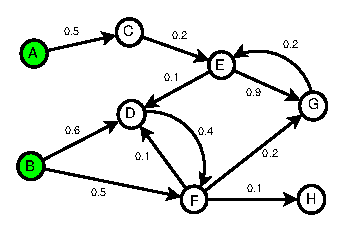
\includegraphics[height=5cm]{algo1.eps}}
    \only<3>{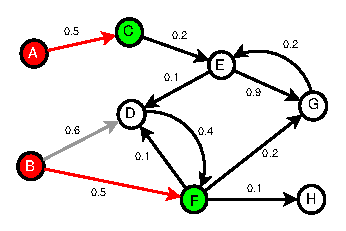
\includegraphics[height=5cm]{algo2.eps}}
    \only<4>{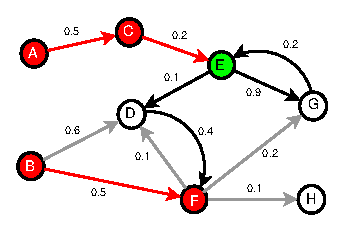
\includegraphics[height=5cm]{algo3.eps}}
    \only<5>{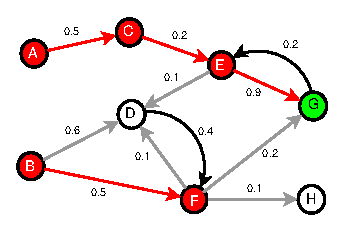
\includegraphics[height=5cm]{algo4.eps}}
    \only<6>{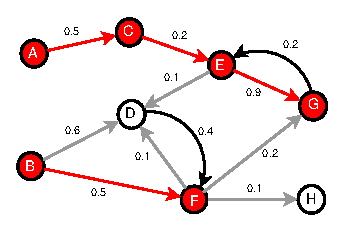
\includegraphics[height=5cm]{algo5.eps}}
  \end{center}
\end{frame}

\begin{frame}{Computing Influence - Live Graph}
  \centering
  \vspace{1em}
  \only<1>{
  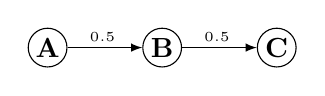
\begin{tikzpicture}
    \draw 
    node[vertex] (A) {A} 
    node[prob, above right=-3pt and 10pt of A] {\tiny $0.5$} 
    node[vertex,right=of A] (B) {B} 
    node[prob, above right=-3pt and 10pt of B] {\tiny $0.5$} 
    node[vertex,right=of B] (C) {C};
    \draw [->] (A) edge (B) (B) edge (C);
  \end{tikzpicture}\\[1em]
  }
  \only<2->{
  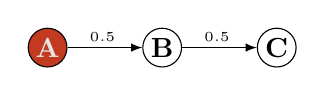
\begin{tikzpicture}
    \draw 
    node[seed] (A) {A} 
    node[prob, above right=-3pt and 10pt of A] {\tiny $0.5$} 
    node[vertex,right=of A] (B) {B} 
    node[prob, above right=-3pt and 10pt of B] {\tiny $0.5$} 
    node[vertex,right=of B] (C) {C};
    \draw [->] (A) edge (B) (B) edge (C);
  \end{tikzpicture}\\[1em]
  }
  \onslide<2->{
  \begin{tabular}{p{5cm}K{1cm}K{1cm}}
    \toprule
    Live Graph ($\mathcal{X}$) & $f_{\mathcal{X}}(\{A\})$ & $P(\mathcal{X})$ \\
    \midrule
    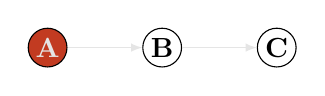
\begin{tikzpicture}
      \draw 
      node[seed] (A) {A} 
      node[vertex,right=of A] (B) {B} 
      node[vertex,right=of B] (C) {C};
      \draw [->,arrowclr] (A) edge (B) (B) edge (C);
    \end{tikzpicture}
     & 1 & $0.25$ \\[0.4em]
    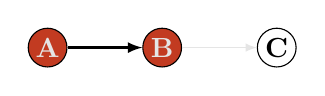
\begin{tikzpicture}
      \draw 
      node[seed] (A) {A} 
      node[seed,right=of A] (B) {B} 
      node[vertex,right=of B] (C) {C};
      \draw [->,thick] (A) edge (B);
      \draw [->,arrowclr] (B) edge (C);
    \end{tikzpicture}
     & 2 & $0.25$ \\[0.4em]
    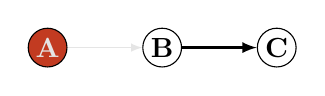
\begin{tikzpicture}
      \draw 
      node[seed] (A) {A} 
      node[vertex,right=of A] (B) {B} 
      node[vertex,right=of B] (C) {C};
      \draw [->,thick] (B) edge (C);
      \draw [->,arrowclr] (A) edge (B);
    \end{tikzpicture}
     & 1 & $0.25$ \\[0.4em]
    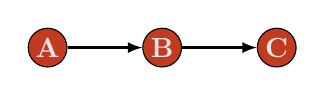
\begin{tikzpicture}
      \draw 
      node[seed] (A) {A} 
      node[seed,right=of A] (B) {B} 
      node[seed,right=of B] (C) {C};
      \draw [->,thick] (A) edge (B) (B) edge (C);
    \end{tikzpicture}
     & 3 & $0.25$ \\
    \bottomrule
  \end{tabular}
  }
  \only<2>{
  \begin{eqnarray*}
    f(\{A\}) & = & \sum_{\mathcal{X}}\mathbf{P}(\mathcal{X})f_{\mathcal{X}}(\{A\}) \\
    & = & 0.25 * ( 1 + 2 + 1 + 3 ) \\
    & = & 1.75 \\
  \end{eqnarray*}
  }
  \onslide<3>{
  \begin{empheq}[box={\tcbhighmath[colback=emphbg]}]{align*}
    \mathsf{P}(\mathcal{X}) & = \prod_{e \in \mathcal{X}} p_{e} \prod_{e \notin \mathcal{X}}(1-p_{e})\\
    f(S) & = \sum_{\mathcal{X}}\mathsf{P}(\mathcal{X})f_{\mathcal{X}}(S)
  \end{empheq}
  }
\end{frame} 

% \begin{frame}{Computing Influence - Live Graph}
%   \begin{center}
%     $f(S)$ : Expected number of active/infected/reached nodes when starting with set $S$
%   \end{center}
%   \begin{itemize}
%     \item A live graph $\mathcal{X}$ is an instance of $G$
%     \pause
%     \item $\forall e \in G$, sample as follows
%     \begin{itemize}
%       \item $\mathsf{P}(e\in \mathcal{X}) = p_e$
%       \item $\mathsf{P}(e\not\in \mathcal{X}) = 1-p_e$
%     \end{itemize}
%     \pause
%     \item Probability of occurrence of live graph $\mathcal{X}$
%     \begin{displaymath}
%       \mathsf{P}(\mathcal{X}) = \prod_{e \in \mathcal{X}} p_{e} \prod_{e \notin \mathcal{X}}(1-p_{e})
%     \end{displaymath}
%     \pause
%     \item Expectation over all live graphs
%     \begin{displaymath}
%       f(S) = \sum_{\mathcal{X}}\mathsf{P}(\mathcal{X})f_{\mathcal{X}}(S)
%     \end{displaymath}
%   \end{itemize}
%%\end{frame}

\section{Relevant Literature and Research Gap}

\begin{frame}{Relevant Literature}
  \begin{itemize}
    \item Influence maximization in a network in a {\color{blue}{single phase using seed nodes}}
    \footnote{\scriptsize D. Kempe, J. Kleinberg, and E. Tardos. Maximizing the spread of influence through a social network. In ACM SIGKDD, pages 137--146, 2003.}
    % \begin{itemize}
    %   \item Function is non-negative, monotone, submodular
    %   \item Greedy hill-climbing gives an approximation factor $(1-\frac{1}{e}-\epsilon)$,
    %     where $\epsilon$ is small for large number of Monte-Carlo simulations
    % \end{itemize}
    % \item Fast heuristics for influence maximization %in the IC model
    % \footnote{\scriptsize W. Chen, Y. Wang, and S. Yang. Efficient influence maximization in social networks. In ACM SIGKDD, pages 199--208. ACM, 2009.}
    % \footnote{\scriptsize A. Guille, H. Hacid, C. Favre, and D. Zighed. Information diffusion in online social networks: A survey. {\em ACM SIGMOD Record}, 42(1):17--28, 2013.}
    % \item An algorithm agnostic to submodularity
    % \footnote{R. Narayanam and Y. Narahari. A shapley value-based approach to discover influential nodes in social networks. IEEE TASE, (99):1-18, 2010.}
    % \item Influence maximization with temporal constraints
    % \footnote{W. Chen, W. Lu, and N. Zhang. Time-critical influence maximization in social networks with time-delayed diffusion process. In AAAI, 592-598, 2012.}
    
    \item Influence maximization using {\color{red}{referral incentives}}
    \footnote{\scriptsize  P. Dayama, A. Karnik, and Y. Narahari. Optimal incentive timing strategies for product marketing on social networks. In AAMAS, pages 703--710, 2012.}
    %\footnote{\scriptsize P. Schmitt, B. Skiera, and C. Van den Bulte. Referral programs and customer value. {\em Journal of Marketing}, 75(1):46–-59, 2011.}
    % \footnote{\scriptsize P. Xiao, C. S. Tang, and J. Wirtz. Optimizing referral reward programs under impression management considerations. {\em EJOR}, 215(3):730–-739, 2011.}
    
    \item Influence maximization in a network {\color{blue}{in two phases using  seed nodes}}
    \footnote{\scriptsize S. Dhamal, K. J. Prabuchandran, and Y. Narahari.  Information diffusion in social networks in two phases. {IEEE TNSE}, 3(4):197--210, 2016.}
    % \footnote{\scriptsize D. Golovin and A. Krause. Adaptive Submodularity: Theory \& Applications in Active Learning and Stochastic Optimization. {\em JAIR}, 42, 427--486, 2011.}
  \end{itemize}
  \vspace{2mm}
  \onslide<2->{
  \begin{empheq}[box={\tcbhighmath[colback=emphbg]}]{align*}
    & \text{Influence maximization with {\color{blue}{budget-split}} in {\color{blue}{two phases}}, using}\\
    & \text{{\color{red}{seed nodes}}, followed by {\color{red}{referral incentives}}}
  \end{empheq}}
\end{frame}

\begin{frame}{Contribution of this Thesis}
\begin{itemize}
\item We formulate a
discrete optimization problem that captures influence maximization 
in two phases using seed nodes and referral incentives

\item We show that the objective
function is non-negative, monotone increasing,
and submodular

\item We conduct simulations on synthetic and real-world network datasets and investigate the following aspects:
\begin{itemize}
\item
How should the total budget be split between the traditional seed selection and referral incentives? 
\item
How does the amount of total available budget affect our budget split?
\item
After how much delay should the second phase be started?
\end{itemize}

\end{itemize}
\end{frame}


\section{Model and Problem Formulation}

\begin{frame}{EXAMPLE K=2, \protect\kn = 1, $\alpha$ = 0.5}
  \centering
  \begin{tabularx}{\linewidth}{CC}
    \addlinespace[1em]
    \multirow{4}{*}{
    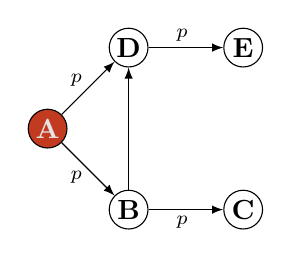
\begin{tikzpicture}
      \draw 
      node[seed] (A) {A} 
      node[prob, above right=10pt and 3pt of A] {\scriptsize $p$} 
      node[vertex,below right=of A] (B) {B} 
      node[prob, below right=-3pt and 12pt of B] {\scriptsize $p$} 
      node[vertex,right=of B] (C) {C} 
      node[prob, below right=10pt and 3pt of A] {\scriptsize $p$} 
      node[vertex,above right=of A] (D) {D} 
      node[prob, above right=-3pt and 12pt of D] {\scriptsize $p$} 
      node[vertex,right=of D] (E) {E};
      \draw [->] (A) edge (B) (B) edge (C) (A) edge (D) (D) edge (E) (B) edge (D);
    \end{tikzpicture}}
    &
    \only<2->{
    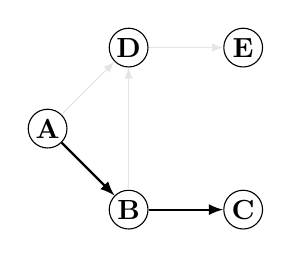
\begin{tikzpicture}
      \draw 
      node[vertex] (A) {A}
      node[vertex, below right=of A] (B) {B}
      node[vertex, right=of B] (C) {C}
      node[vertex, above right=of A] (D) {D}
      node[vertex, right=of D] (E) {E};
      \draw [thick,->] (A) edge (B) (B) edge (C);
      \draw [txtclr,->] (A) edge (D) (D) edge (E) (B) edge (D);
    \end{tikzpicture}
    \\
    & ~~~~~~~~~Live Graph}\\
    \addlinespace[2em]
    &
    \only<3> {
    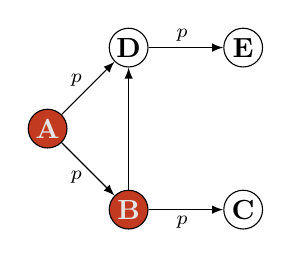
\begin{tikzpicture}
      \draw 
      node[seed] (A) {A} 
      node[prob, above right=10pt and 3pt of A] {\scriptsize $p$} 
      node[seed,below right=of A] (B) {B} 
      node[prob, below right=-3pt and 12pt of B] {\scriptsize $p$} 
      node[vertex,right=of B] (C) {C} 
      node[prob, below right=10pt and 3pt of A] {\scriptsize $p$} 
      node[vertex,above right=of A] (D) {D} 
      node[prob, above right=-3pt and 12pt of D] {\scriptsize $p$} 
      node[vertex,right=of D] (E) {E};
      \draw [->] (A) edge (B) (B) edge (C) (A) edge (D) (D) edge (E) (B) edge (D);
    \end{tikzpicture}\\
    }
    \only<4>{
    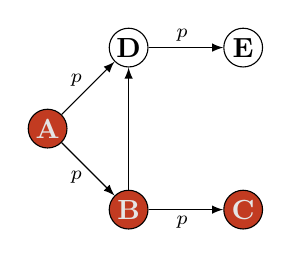
\begin{tikzpicture}
      \draw 
      node[seed] (A) {A} 
      node[prob, above right=10pt and 3pt of A] {\scriptsize $p$} 
      node[seed,below right=of A] (B) {B} 
      node[prob, below right=-3pt and 12pt of B] {\scriptsize $p$} 
      node[seed,right=of B] (C) {C} 
      node[prob, below right=10pt and 3pt of A] {\scriptsize $p$} 
      node[vertex,above right=of A] (D) {D} 
      node[prob, above right=-3pt and 12pt of D] {\scriptsize $p$} 
      node[vertex,right=of D] (E) {E};
      \draw [->] (A) edge (B) (B) edge (C) (A) edge (D) (D) edge (E) (B) edge (D);
    \end{tikzpicture}\\
    }
    \only<3->{
    & ~~~~~~~~~Phase 1 \\}
  \end{tabularx}
\end{frame}

\begin{frame}{2-PHASE MODEL WITH REFERRALS}
  \centering
  \begin{tabularx}{\linewidth}{C|CC}
    \textbf{Phase} $\mathbf{1}$ $\mathbf{(k=1)}$ & \multicolumn{2}{c}{\textbf{Phase} $\mathbf{2}$ $\mathbf{(\alpha=\tfrac{1}{2})}$} \\[1em]
    \raisebox{-.5\height}{
    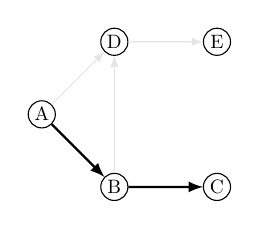
\begin{tikzpicture}[scale=0.7, every node/.style={scale=0.7}]
      \draw 
      node[vertex] (A) {A}
      node[vertex, below right=of A] (B) {B}
      node[vertex, right=of B] (C) {C}
      node[vertex, above right=of A] (D) {D}
      node[vertex, right=of D] (E) {E};
      \draw [thick,->] (A) edge (B) (B) edge (C);
      \draw [txtclr,->] (A) edge (D) (D) edge (E) (B) edge (D);
    \end{tikzpicture}}
    & \only<2->{
    \raisebox{-.5\height}{
    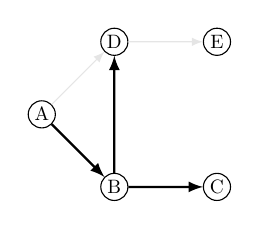
\begin{tikzpicture}[scale=0.7, every node/.style={scale=0.7}]
      \draw 
      node[vertex] (A) {A}
      node[vertex, below right=of A] (B) {B}
      node[vertex, right=of B] (C) {C}
      node[vertex, above right=of A] (D) {D}
      node[vertex, right=of D] (E) {E};
      \draw [thick,->] (A) edge (B) (B) edge (C) (B) edge (D);
      \draw [txtclr,->] (A) edge (D) (D) edge (E);
    \end{tikzpicture}}}
    & \only<5->{
    \raisebox{-.5\height}{
    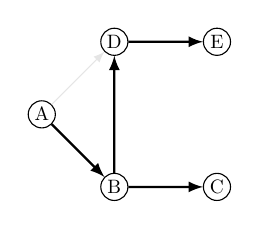
\begin{tikzpicture}[scale=0.7, every node/.style={scale=0.7}]
      \draw 
      node[vertex] (A) {A}
      node[vertex, below right=of A] (B) {B}
      node[vertex, right=of B] (C) {C}
      node[vertex, above right=of A] (D) {D}
      node[vertex, right=of D] (E) {E};
      \draw [thick,->] (A) edge (B) (B) edge (C) (B) edge (D) (D) edge (E);
      \draw [txtclr,->] (A) edge (D);
    \end{tikzpicture}}}
    \\[3em]
    ~~~~~~~~$\mathcal{X}$ & \only<2->{~~~~~~~~$\mathcal{Y}_1|\mathcal{X}$} & \only<5->{~~~~~~~~$\mathcal{Y}_2|\mathcal{X}$}
    \\[1em]
    \raisebox{-.5\height}{
    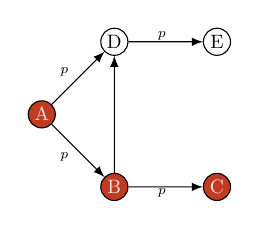
\begin{tikzpicture}[scale=0.7, every node/.style={scale=0.7}]
      \draw 
      node[seed] (A) {A} 
      node[prob, above right=10pt and 3pt of A] {\scriptsize $p$} 
      node[seed,below right=of A] (B) {B} 
      node[prob, below right=-3pt and 12pt of B] {\scriptsize $p$} 
      node[seed,right=of B] (C) {C} 
      node[prob, below right=10pt and 3pt of A] {\scriptsize $p$} 
      node[vertex,above right=of A] (D) {D} 
      node[prob, above right=-3pt and 12pt of D] {\scriptsize $p$} 
      node[vertex,right=of D] (E) {E};
      \draw [->] (A) edge (B) (B) edge (C) (A) edge (D) (D) edge (E) (B) edge (D);
    \end{tikzpicture}}
    & \only<3>{
    \raisebox{-.5\height}{
    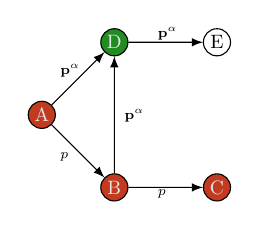
\begin{tikzpicture}[scale=0.7, every node/.style={scale=0.7}]
      \draw 
      node[seed] (A) {A} 
      node[prob, above right=10pt and 3pt of A] {\scriptsize $\mathbf{p^{\alpha}}$} 
      node[seed,below right=of A] (B) {B} 
      node[prob, below right=-3pt and 12pt of B] {\scriptsize $p$} 
      node[seed,right=of B] (C) {C} 
      node[prob, below right=10pt and 3pt of A] {\scriptsize $p$} 
      node[ref,above right=of A] (D) {D} 
      node[prob, above right=-3pt and 12pt of D] {\scriptsize $\mathbf{p^{\alpha}}$} 
      node[vertex,right=of D] (E) {E}
      node[prob, above right=20pt and 0pt of B] {\scriptsize $\mathbf{p^{\alpha}}$};
      \draw [->] (A) edge (B) (B) edge (C) (A) edge (D) (D) edge (E) (B) edge (D);
    \end{tikzpicture}}}
    \only<4->{
    \raisebox{-.5\height}{
    \begin{tikzpicture}[scale=0.7, every node/.style={scale=0.7}]
      \draw 
      node[seed] (A) {A} 
      node[prob, above right=10pt and 3pt of A] {\scriptsize $\mathbf{p^{\alpha}}$} 
      node[seed,below right=of A] (B) {B} 
      node[prob, below right=-3pt and 12pt of B] {\scriptsize $p$} 
      node[seed,right=of B] (C) {C} 
      node[prob, below right=10pt and 3pt of A] {\scriptsize $p$} 
      node[ref,above right=of A] (D) {D} 
      node[prob, above right=-3pt and 12pt of D] {\scriptsize $\mathbf{p^{\alpha}}$} 
      node[vertex,right=of D] (E) {E}
      node[prob, above right=20pt and 0pt of B] {\scriptsize $\mathbf{p^{\alpha}}$}
      node[below=-2pt of B] {
\includegraphics[scale=0.02]{moneybag.png}}
      node[above=-2pt of D] {
\includegraphics[scale=0.02]{moneybag.png}};
      \draw [->] (A) edge (B) (B) edge (C) (A) edge (D) (D) edge (E) (B) edge (D);
    \end{tikzpicture}}}
    & \only<6>{
    \raisebox{-.5\height}{
    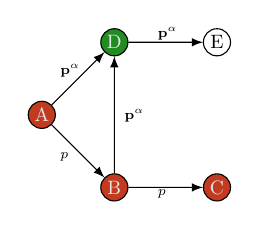
\begin{tikzpicture}[scale=0.7, every node/.style={scale=0.7}]
      \draw 
      node[seed] (A) {A} 
      node[prob, above right=10pt and 3pt of A] {\scriptsize $\mathbf{p^{\alpha}}$} 
      node[seed,below right=of A] (B) {B} 
      node[prob, below right=-3pt and 12pt of B] {\scriptsize $p$} 
      node[seed,right=of B] (C) {C} 
      node[prob, below right=10pt and 3pt of A] {\scriptsize $p$} 
      node[ref,above right=of A] (D) {D} 
      node[prob, above right=-3pt and 12pt of D] {\scriptsize $\mathbf{p^{\alpha}}$}
      node[vertex,right=of D] (E) {E}
      node[prob, above right=20pt and 0pt of B] {\scriptsize $\mathbf{p^{\alpha}}$};
      \draw [->] (A) edge (B) (B) edge (C) (A) edge (D) (D) edge (E) (B) edge (D);
    \end{tikzpicture}}} 
    \only<7>{
    \raisebox{-.5\height}{
    \begin{tikzpicture}[scale=0.7, every node/.style={scale=0.7}]
      \draw 
      node[seed] (A) {A} 
      node[prob, above right=10pt and 3pt of A] {\scriptsize $\mathbf{p^{\alpha}}$} 
      node[seed,below right=of A] (B) {B} 
      node[prob, below right=-3pt and 12pt of B] {\scriptsize $p$} 
      node[seed,right=of B] (C) {C} 
      node[prob, below right=10pt and 3pt of A] {\scriptsize $p$} 
      node[ref,above right=of A] (D) {D} 
      node[prob, above right=-3pt and 12pt of D] {\scriptsize $\mathbf{p^{\alpha}}$}
      node[vertex,right=of D] (E) {E}
      node[prob, above right=20pt and 0pt of B] {\scriptsize $\mathbf{p^{\alpha}}$}
      node[below=-2pt of B] {
\includegraphics[scale=0.02]{moneybag.png}}
      node[above=-2pt of D] {
\includegraphics[scale=0.02]{moneybag.png}};
      \draw [->] (A) edge (B) (B) edge (C) (A) edge (D) (D) edge (E) (B) edge (D);
    \end{tikzpicture}}}
    \only<8>{
    \raisebox{-.5\height}{
    \begin{tikzpicture}[scale=0.7, every node/.style={scale=0.7}]
      \draw 
      node[seed] (A) {A} 
      node[prob, above right=10pt and 3pt of A] {\scriptsize $\mathbf{p^{\alpha}}$} 
      node[seed,below right=of A] (B) {B} 
      node[prob, below right=-3pt and 12pt of B] {\scriptsize $p$} 
      node[seed,right=of B] (C) {C} 
      node[prob, below right=10pt and 3pt of A] {\scriptsize $p$} 
      node[ref,above right=of A] (D) {D} 
      node[prob, above right=-3pt and 12pt of D] {\scriptsize $\mathbf{p^{\alpha}}$}
      node[ref,right=of D] (E) {E}
      node[prob, above right=20pt and 0pt of B] {\scriptsize $\mathbf{p^{\alpha}}$}
      node[below=-2pt of B] {
\includegraphics[scale=0.02]{moneybag.png}}
      node[above=-2pt of D] {
\includegraphics[scale=0.02]{moneybag.png}};
      \draw [->] (A) edge (B) (B) edge (C) (A) edge (D) (D) edge (E) (B) edge (D);
    \end{tikzpicture}}}
    \only<9->{
    \raisebox{-.5\height}{
    \begin{tikzpicture}[scale=0.7, every node/.style={scale=0.7}]
      \draw 
      node[seed] (A) {A} 
      node[prob, above right=10pt and 3pt of A] {\scriptsize $\mathbf{p^{\alpha}}$} 
      node[seed,below right=of A] (B) {B} 
      node[prob, below right=-3pt and 12pt of B] {\scriptsize $p$} 
      node[seed,right=of B] (C) {C} 
      node[prob, below right=10pt and 3pt of A] {\scriptsize $p$} 
      node[ref,above right=of A] (D) {D} 
      node[prob, above right=-3pt and 12pt of D] {\scriptsize $\mathbf{p^{\alpha}}$}
      node[ref,right=of D] (E) {E}
      node[prob, above right=20pt and 0pt of B] {\scriptsize $\mathbf{p^{\alpha}}$}
      node[below=-2pt of B] {
\includegraphics[scale=0.02]{moneybag.png}}
      node[above=-2pt of D] {
\includegraphics[scale=0.02]{moneybag.png}
\includegraphics[scale=0.02]{moneybag.png}}
      node[above=-2pt of E] {
\includegraphics[scale=0.02]{moneybag.png}};
      \draw [->] (A) edge (B) (B) edge (C) (A) edge (D) (D) edge (E) (B) edge (D);
    \end{tikzpicture}}}
    \\
    & \only<4->{~~~~~~~~
\includegraphics[scale=0.02]{tick.png}} & \only<10>{~~~~~~~~
\includegraphics[scale=0.09]{cross.png}} \\
  \end{tabularx}
\end{frame}

\begin{frame}{Effect of $\alpha$}

\onslide<1->{
  \begin{center}
    {\color{blue}{How to capture effect of }}{\color{red}{$\alpha$-reward}}{\color{blue}{?}}
  \end{center}
}
\onslide<2->{
  \begin{itemize}
    \item Incentive to individual nodes
    \item Overall edge influence probabilities expected to increase!
  \end{itemize}
  }
\onslide<3->{
  \begin{empheq}[box={\tcbhighmath[colback=emphbg]}]{align*}
    & {\color{red}{\mathbf{h(\alpha)}}} \text{{\color{blue}{ : fractional increase in edge influence probability}}}
  \end{empheq}
}

\begin{itemize}
\onslide<4->{
    \item non-negative
    \item no reward $\implies$ no increase in probability; $h(0) = 0$
    \item non-decreasing in [0,1]
}
\onslide<5->{
    \item $h(\alpha) = log(1+\alpha)$ \\
    \only<5>{
    $p^\alpha = (1+log(1+\alpha))p$}
    \only<6>{
    $p^\alpha = \min\{1, (1+log(1+\alpha))p$\}}
}
    \end{itemize}   
\end{frame}



% \begin{frame}{Notation}
%   \begin{itemize}
%     \item \color{red}{$K$} = total available budget
%     \pause
%     \item \color{red}{$(k,\alpha)$} - split
%     \begin{itemize}
%       \item $S^k$ : seed set for phase 1
%       \item $\alpha$ : percentage reward for phase 2
%     \end{itemize}
%     \item \color{red}{$h(\alpha)$} = fractional increase in influence probability
%     \begin{itemize}
%       \item $p_{uv} \rightarrow p_{uv}^{\alpha} = min {(1+h(\alpha))p_{uv},1}$
%       \item $h(\alpha)$ is monotone, non-decreasing, continuous in [0,1]
%       \item $h(0) = 0$
%     \end{itemize}
%     \item \color{red}{$f(k,\alpha$)} = influence function with $(k,\alpha)$ split
%   \end{itemize}
% \end{frame}

% \begin{frame}{Proposed Model}
%   \hspace{-6mm}
%   \begin{tabular}{|p{0.35\textwidth}|p{0.64\textwidth}|}
%     \hline
%     ~Phase One - Diffusion & ~~~~~~~ Phase Two - Referral Rewards\\
%     \hline
%     \begin{itemize}
%       \item $k$ free samples
%       \item Select optimal seed set $S^{k}$
%       \item Diffusion until termination
%       \item Set of current active nodes $A_{diff}$
%       \item Remaining budget = $K-k$
%     \end{itemize}
%     &
%     \onslide<2->{
%     \begin{itemize}
%       \item Inactive set $\bar{A}_{diff} = V\setminus A_{diff}$ %\newline
%       \item $\forall j \in \bar{A}_{diff}$, let $N(j) = \{i | p_{i,j} > 0; i \in A_{diff}\}$ \newline (set of node $j$'s active neighbours)
%       \item \textit{Scaled} $P(i \rightarrow j) = \epsilon_\alpha p_{i,j} \in [0,1]; \epsilon_{\alpha} \geq 1$
%       \item If referral successful, award $\alpha$ to node $i$, \newline
%       $A_d = A_d \cup \{j\}$, $\bar{A}_d = \bar{A}_d\setminus\{j\}$
%       \item Newly activated set $A_{r}$, live graph $\mathcal{X}$
%     \end{itemize}
%     }\\
%     \hline
%   \end{tabular}
% \end{frame}

% \begin{frame}{Proposed Model}
%   \begin{columns}
%     \column{0.35\textwidth}
%     \begin{block}{Phase One - Diffusion}
%       \begin{itemize}
%         \item $k$ free samples
%         \item Select optimal seed set $S^{k}$
%         \item Diffusion until termination
%         \item Set of current active nodes $A_{diff}$
%         \item Remaining budget = $K-k$
%       \end{itemize}
%     \end{block}
%     \pause
%     \column{0.69\textwidth}
%     \begin{block}{   Phase Two - Referral Rewards}
%       \begin{itemize}
%         \item Inactive set $\bar{A}_{diff} = V\setminus A_{diff}$ \\
%         \item $\forall j \in \bar{A}_{diff}$, let $N(j) = \{i | p_{i,j} > 0; i \in A_{diff}\}$ \\(set of node $j$'s active neighbours)
%         \item \textit{Scaled} $P(i \rightarrow j) = \epsilon_\alpha p_{i,j} \in [0,1]; \epsilon_{\alpha} \geq 1$
%         \item If referral successful, award $\alpha$ to node $i$, \\
%         $A_d = A_d \cup \{j\}$, $\bar{A}_d = \bar{A}_d\setminus\{j\}$
%         \item Newly activated set $A_{r}$, live graph $\mathcal{X}$
%       \end{itemize}
%     \end{block}
%   \end{columns}
% \end{frame}

% \begin{frame}{Influence Function (CONTD...)}
%   \begin{itemize}
%     \item $\mathcal{X}$ : Live graph obtained after phase 1\\
%     \begin{center}
%       $p(\mathcal{X}) = \prod_{(u,v) \in \mathcal{X}}p_{{uv}}\prod_{(u,v) \notin \mathcal{X}} (1-p_{{uv}})$
%     \end{center}
%     \pause
%     \item $\mathcal{Y}$ : Live graph obtained after phase 2\\
%     \begin{center}
%       $p(\mathcal{Y}|\mathcal{X};\alpha) = \prod_{(u,v) \in \mathcal{Y}\setminus \mathcal{X}} \left( \frac{p_{uv}^\alpha - p_{uv}}{1-p_{uv}} \right) \prod_{(u,v) \notin \mathcal{Y}} \left( \frac{1-p_{uv}^\alpha}{1-p_{uv}} \right)$
%     \end{center}
%     \item $A_{diff}^{\mathcal{X}}$ = Nodes active after phase 1
%     \begin{center}
%       $A_{diff}^{\mathcal{X}} = \{v|\text{ } v \text{ is reachable from }S^k \text{ in } \mathcal{X}\}$
%     \end{center}
%     \item $A_{ref}^{\mathcal{Y}}$ = Additional nodes activated in phase 2
%     \begin{center}
%       $A_{ref}^{\mathcal{Y}} = \{v|\text{ } v \text{ is reachable from }A_{diff}^{\mathcal{X}} \text{ in } \mathcal{Y}\} \setminus A_{diff}^{\mathcal{X}}$
%     \end{center}
%     \item $f(S^k,\alpha)$ = Expected number of influenced nodes
%     \begin{center}
%       $f(S^k,\alpha) = \sum_{\mathcal{X}}p(\mathcal{X}) \left\lbrace|A_{diff}^{\mathcal{X}}| + \sum_{\mathcal{Y}}p(\mathcal{Y}|\mathcal{X};\alpha)|A_{ref}^{\mathcal{Y}}|\right\rbrace$
%     \end{center}
%   \end{itemize}
% \end{frame}

\begin{frame}{Optimization Problem}
  \begin{equation*}
    \label{opt_problem}
    \begin{array}{|c|}
      \hline\\
      \text{Select } (S_k,\alpha) \text{ to give}\\ \\
      \max\limits_{\substack{\mathbf{k \leq K, \alpha \in [0,1]} \\ \mathbf{S_k \subset V}}} f(S_k,\alpha) = \underbrace{\mathbb{E}\left[|A_{diff}(S_k)|\right]}_{\text{\color{red}{depends on $k$}}} + \underbrace{\mathbb{E}\left[|A_{ref}(S_k;\alpha)|\right]}_{\text{\color{blue}{depends on $k,h(\alpha)$}}} \\ \\ \\
      
%       \mathbb{E}^\mathcal{X} \Big[|A_{diff}(S_k)| + \mathbb{E}^{\mathcal{Y}|\mathcal{X};\alpha} \left[|A_{ref}(S_k;\alpha)|\right] \Big]
%       \\ \\
% \text{subject to } \\ \\
%       \mathbb{E}^\mathcal{X} \mathbb{E}^{\mathcal{Y}|\mathcal{X};\alpha} \left[|A_{ref}(S^k;\alpha)|\right] \leq \frac{K-k}{2\alpha} \\ \\
      %
%       f(S^k,\alpha) = \sum_{\mathcal{X}}p(\mathcal{X}) \left\lbrace|A_{diff}^{\mathcal{X}}| + \sum_{\mathcal{Y}}p(\mathcal{Y}|\mathcal{X};\alpha)|A_{ref}^{\mathcal{Y}}|\right\rbrace \\ \\
      \text{subject to } \\ \\
      \mathbb{E}\left[|A_{ref}(S^k;\alpha)|\right] \leq \frac{K-k}{2\alpha} \\ \\
      \hline
    \end{array}
  \end{equation*}
\end{frame}

\begin{frame}{Properties of Influence Function}
$f(S_k,\alpha)$ is:
\begin{itemize}
\item non-negative
\item monotone increasing
\item sub-modular
\end{itemize}

\end{frame}

\begin{frame}{Algorithm - Modified Greedy}
\begin{algorithm}[H]
\begin{small}
\DontPrintSemicolon
\KwIn{Graph $G$, budget $K$, split $(k,\alpha)$}
\KwOut{Optimal seed set $S_k$ such that $|S_k|\leq k$}
%\textbf{Initialize:} $\alpha_{i,1} = 0 , \beta_{i,1} = 0 \  \forall i \in \{1,2, \ldots, k\}$\\
$S_k \gets \phi$
\\
\For{$t \gets 1$ \textbf{to} $k$}{
\For{$v \notin S_k$}{
\only<1>{
Compute $f(S_k \cup \{v\})$ \;
}
\only<2>{
{\color{red}{Compute $f(S_k \cup \{v\})$}} \;
}
}
\only<1>{
$V_{valid} \gets \left\{ v \in V \setminus S_k : \mathbb{E}|A_{ref}(S_k \cup \{v\})| \leq \frac{K-k}{2\alpha}\right\}$ \;
}
\only<2>{
{\color{red}{
$V_{valid} \gets \left\{ v \in V \setminus S_k : \mathbb{E}|A_{ref}(S_k \cup \{v\})| \leq \frac{K-k}{2\alpha}\right\}$}} \;
}
\vspace{2mm}
$v_t \gets \argmax_{v \in V_{valid}} f(S_k \cup \{v\}) - f(S_k)$  %\hfill[breaking ties randomly]\;

\vspace{2mm}
\If{$\{v_t\} \neq \phi$}{
$S_k \gets S_k \cup \{v_t\}$ \;
}
\Else{return $S_k$ \hfill[{\color{blue}{$|S_k| < k$}}]\;}
}
\end{small}
\caption{A modified greedy algorithm for seed selection}
%\label{alg:modified_greedy}
\end{algorithm}
\end{frame}


\section{Experimental Evaluation}

\begin{frame}{datasets}
\begin{itemize}
\item Les Miserables
\begin{itemize}
\item {\color{blue}{77}} nodes, {\color{blue}{254}} undirected edges
\item {Suitable for running time and memory intensive algorithms}
\end{itemize}
 \vspace{10mm}
 \pause
\item NetHEPT 
\begin{itemize}
\item {\color{blue}{15233}} nodes, {\color{blue}{31398}} undirected edges
\item Exhibits most structural properties of ``social-network" graphs
\end{itemize}
\end{itemize}
\end{frame}

\begin{frame}{Performance of 2-Phase vs. single-phase}
  \begin{center}
    \only<1>{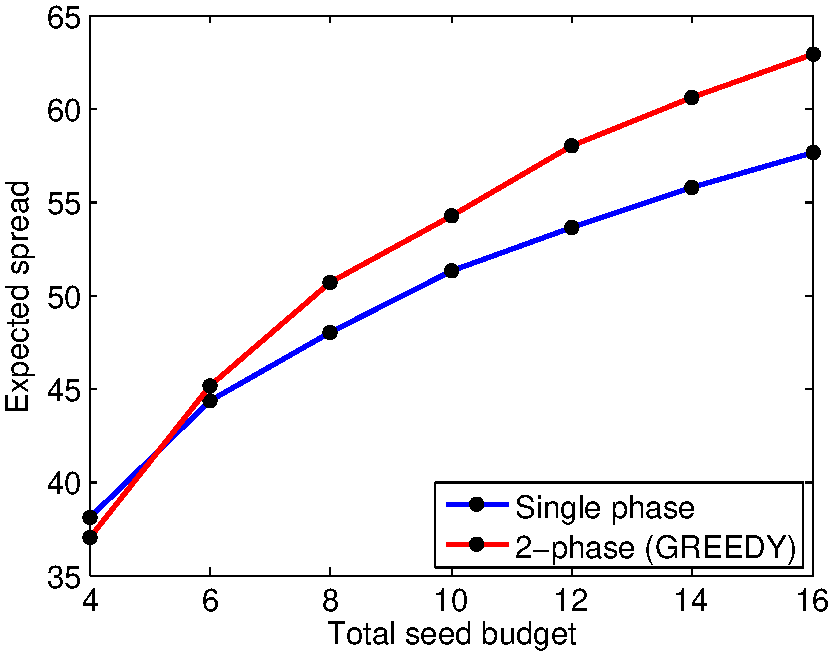
\includegraphics[height= 4.5cm]{LM_1_cropped.pdf}   }
  \end{center}
  %{\color{blue}{Observations}}:
  \begin{itemize}  
  	\item Budget-split detrimental for small $K$, yields significant gains for moderate-high $K$, relative gain increases with $K$
      
  \end{itemize}
\end{frame}

\begin{frame}{Performance of 2-Phase vs. single-phase (Les Miserables)}
  \begin{center}
    \only<1>{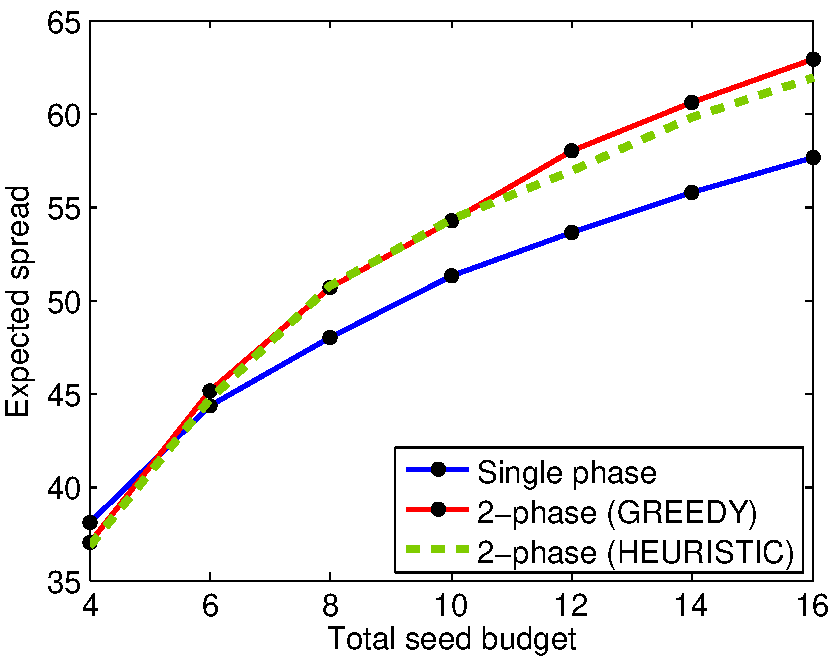
\includegraphics[height= 4.5cm]{LM_2_cropped.pdf}   }
  \end{center}
  %{\color{blue}{Observations}}:
  \begin{itemize}  
  	\item Budget-split detrimental for small $K$, yields significant gains for moderate-high $K$
    \item PMIA heuristic performs nearly as well as 2-phase greedy
    
  \end{itemize}
\end{frame}

\begin{frame}{Effect of \protect\kn,$\alpha$}
  \begin{center}
    \vspace{-5mm}
    \begin{tabular}{cc}
      %\hline
      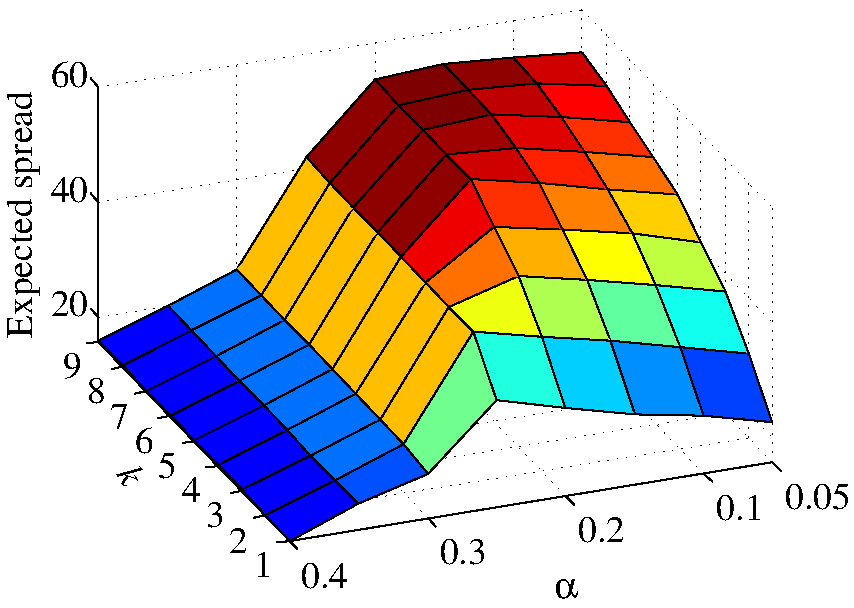
\includegraphics[height = 3.7cm]{LM_3d_plot_cropped.pdf}
      &
      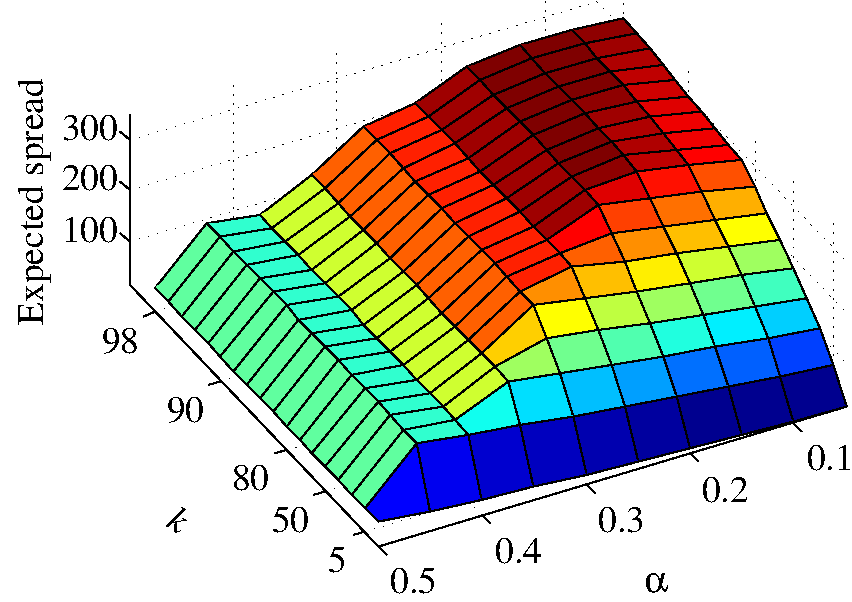
\includegraphics[height = 3.7cm]{Coverage_3d_TV_cropped.pdf}
      \\ %\hline
      LM ($K=10$)
      &
      NetHEPT ($K=100$)
      \\ %\hline
    \end{tabular}
  \end{center}
  \pause
  %Observations :
  \begin{itemize}
    \item Maximum spread observed at {\color{red}{high}} $k$, {\color{red}{low}} $\alpha$ pairs\\
    Optimal split for LM : {\color{blue}{(7, 0.15)}}. Gain $\approx$ {\color{blue}{6\%}}
    \\
    Optimal split for NetHEPT : {\color{blue}{(82, 0.15)}}. Gain $\approx$  {\color{blue}{7\%}}
    \pause 
    \\
    {\color{blue}{WHY?}}\\
    \pause
	
    Need enough active nodes after phase 1 to act as {\color{red}{referring agents}} for phase 2!
    \end{itemize}
\end{frame}

\begin{frame}{Effect of \protect\kn,$\alpha$}
  \begin{center}
    \vspace{-5mm}
    \begin{tabular}{cc}
      %\hline
      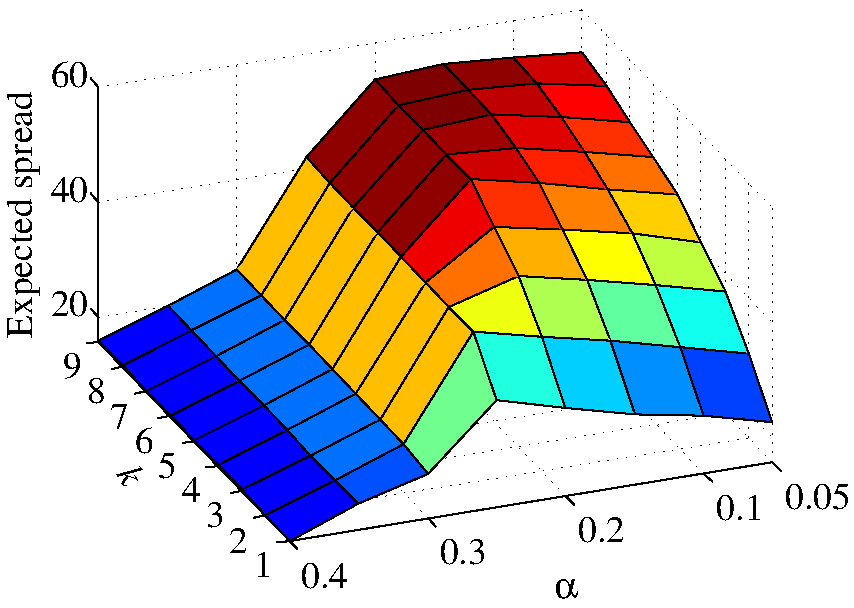
\includegraphics[height = 3.7cm]{LM_3d_plot_cropped.pdf}
      &
      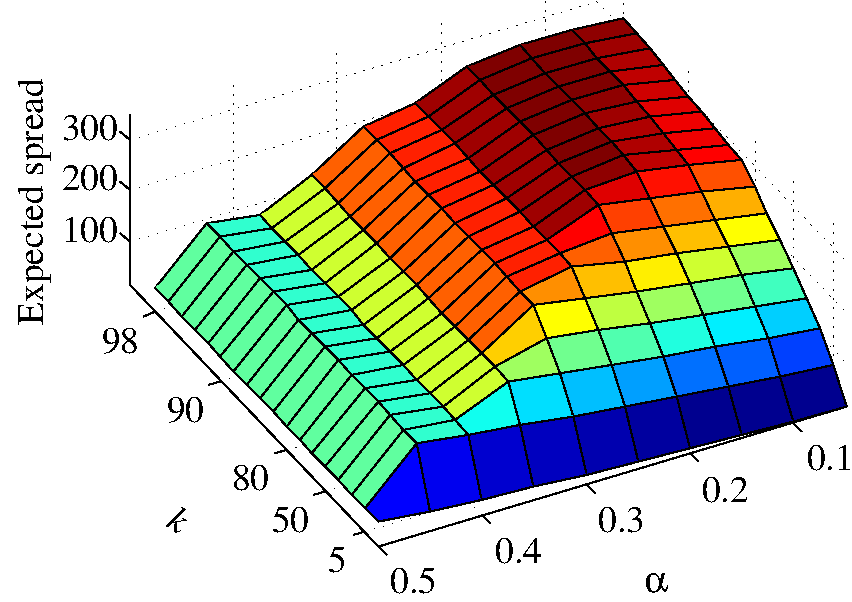
\includegraphics[height = 3.7cm]{Coverage_3d_TV_cropped.pdf}
      \\ %\hline
      LM ($K=10$)
      &
      NetHEPT ($K=100$)
      \\ %\hline
    \end{tabular}
  \end{center}
  %Observations :
  \begin{itemize}
    \item Maximum spread observed at {\color{red}{high}} $k$, {\color{red}{low}} $\alpha$ pairs\\
    \item Improved spread {\color{red}{never}} attained at very high $\alpha$ \\
    \pause
    {\color{blue}{WHY}?} \\
    \pause
    Higher $\alpha$ $\implies$ fewer permissible active nodes in phase 2!
  \end{itemize}
\end{frame}

\begin{frame}{Temporal Progression of 2-phase model}
  \begin{center}
    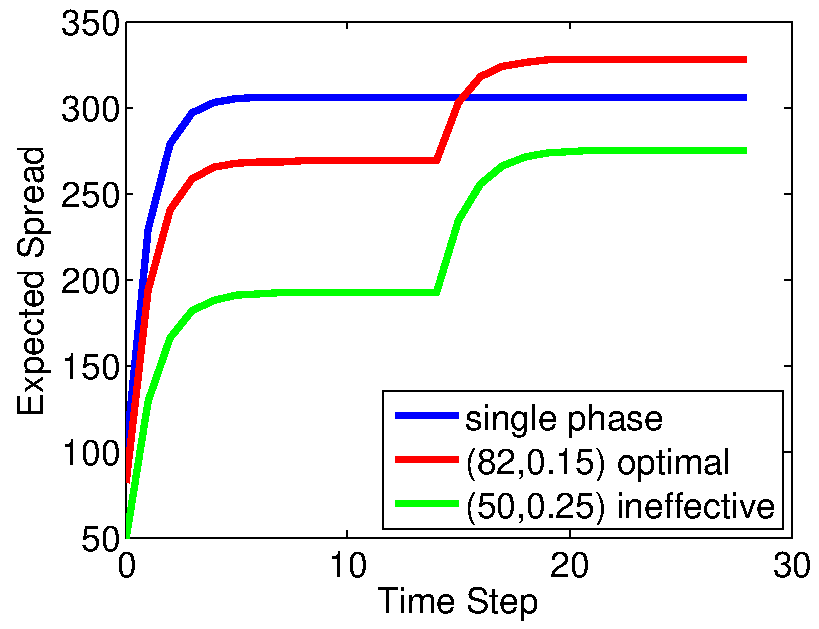
\includegraphics[height = 4.5cm]{time_lapse_cropped.pdf}
    \\
    {  NetHEPT ($K = 100$)}
  \end{center}
  \begin{itemize}
  \item Single phase saturates earliest
  \item Two-phase saturates after phase 1, shoots up on initiating phase 2
  \item Allocating sufficient budget for phase 1 is crucial!
  \end{itemize}
\end{frame}

\section{Summary and Future Work}

\begin{frame}{Summary and Future Work}
  \begin{itemize}
  \item In conclusion, we have:
  \begin{itemize}
  \item Proposed a referral incentive based model
  \item Analysed the mathematical properties of said model
  \item Studied efficacy of the model on real-life datasets
  \end{itemize}
  \pause
  \item{Future Work}
  \end{itemize}
\end{frame}

\begin{frame}{Publication Based on this Thesis}
  \begin{itemize}
  \item
  Sneha Mondal, Swapnil Dhamal, and Y. Narahari. Two-Phase Influence Maximization in Social Networks with Seed Nodes and Referral Incentives. \\
  \vspace{3mm}
  The 10th International Workshop on Mining Actionable Insights from Social Networks (MAISoN). To appear, Cambridge, UK. ACM, 2017.
  \end{itemize}
\end{frame}

\end{document} 